\documentclass[crop,tikz]{standalone}
\usetikzlibrary{calc}
\usetikzlibrary{arrows}
\usetikzlibrary{decorations.pathreplacing}
\begin{document}
\begin{tikzpicture}
  % Constants
  \pgfmathsetmacro\b{9}
  \pgfmathsetmacro\n{13}
  \pgfmathsetmacro\d{110.45}
  \pgfmathsetmacro\c{95.62}
  \pgfmathsetmacro\t{2}
  \pgfmathsetmacro\a{0}
  %% \pgfmathsetmacro\ox{\c*cos(\a+\t)}
  %% \pgfmathsetmacro\oy{\c*sin(\a)}
  \pgfmathsetmacro\ox{0}
  \pgfmathsetmacro\oy{0}
  % Boundary
  \path[use as bounding box] (0,0) rectangle (\n*\b+2,\b+2);
  % Domain grids
  \foreach \i in {1,...,\n}{
    \draw ({1+(\i-1)*\b},1) -- (\i*\b+1,1) -- (\i*\b+1,\b+1) -- ({1+(\i-1)*\b},\b+1) -- cycle;
  }
  % Lightcone
  \begin{scope}[shift={(1-\ox,1-\oy)}]
    %% \clip (\ox,\oy) rectangle(\b+\ox,\b+\oy);
    \filldraw[fill=blue,fill opacity=0.1,draw=blue!90] (\a:\c) arc (\a:\a+\t:\c) -- (\a+\t:\d) arc (\a+\t:\a:\d) -- cycle;
  \end{scope}
  %% \begin{scope}[shift={(1-\b-\ox,1-\oy)}]
  %%   \clip (\b+\ox,\oy) rectangle(2*\b+\ox,\b+\oy);
  %%   \filldraw[fill=blue,fill opacity=0.1,draw=blue!90] (\a:\c) arc (\a:\a+\t:\c) -- (\a+\t:\d) arc (\a+\t:\a:\d) -- cycle;
  %% \end{scope}
  %% \begin{scope}[shift={(1-2*\b,1)}]
  %%   \clip (2*\b,0) rectangle(3*\b,\b);
  %%   \filldraw[fill=blue,fill opacity=0.1,draw=blue!90] (\a:\c) arc (\a:\a+\t:\c) -- (\a+\t:\d) arc (\a+\t:\a:\d) -- cycle;
  %%   %% \filldraw[fill=blue,fill opacity=0.1,draw=blue!90] (0,0) -- (\a:\d) arc (\a:\a+\t:\d) -- cycle;
  %% \end{scope}
\end{tikzpicture}
\end{document}
